% =============================================================
% InsightOps AI: A Governed Multi-Agent ChatBI Platform
% IEEEtran conference-style report
%
% EDIT-ME PLACEHOLDERS (search for "TODO"):
%   - Author email (currently shanhaoyuan820712@gmail.com)
%   - Affiliation / course line (currently mirrors the EraseGraph
%     report's SJSU MSSE affiliation; change if this submission is
%     for a different course/instructor)
% =============================================================
\documentclass[conference]{IEEEtran}
\IEEEoverridecommandlockouts

\usepackage{cite}
\usepackage{amsmath,amssymb,amsfonts}
\usepackage{graphicx}
\usepackage{textcomp}
\usepackage{xcolor}
\usepackage{booktabs}
\usepackage{array}
\usepackage{tikz}
\usetikzlibrary{arrows.meta, positioning, shapes.geometric, fit, backgrounds}
\usepackage[hidelinks]{hyperref}

\def\BibTeX{{\rm B\kern-.05em{\sc i\kern-.025em b}\kern-.08em
    T\kern-.1667em\lower.7ex\hbox{E}\kern-.125emX}}

\begin{document}

\title{InsightOps AI: A Governed Multi-Agent ChatBI Platform for Enterprise Decision Intelligence}

\author{
\IEEEauthorblockN{Haoyuan Shan}
\IEEEauthorblockA{
Master's in Software Engineering \\
San Jose State University \\ % TODO: confirm affiliation/course line
San Jose, United States \\
shanhaoyuan820712@gmail.com % TODO: confirm submission email
}
}

\maketitle

\begin{abstract}
Most enterprise business-intelligence systems are either static dashboards or
analyst-driven SQL workflows, which leaves business users waiting on a data
team for every follow-up question. Asking a large language model to write
and run SQL directly does not solve this: an ungoverned model can reference
the wrong table, leak sensitive fields, or simply hallucinate a plausible
but wrong answer. In this project we built InsightOps AI, a governed
multi-agent ChatBI platform that treats a natural-language business
question as a workflow, not a single model call. A router classifies the
question, a semantic layer constrains what the model may reference, a
non-LLM SQL guardrail validates and rewrites every generated SQL candidate
before it is allowed to reach a database-level read-only role, a hybrid
retrieval pipeline (BM25 keyword scoring fused with real embeddings and an
optional cross-encoder rerank stage, backed by pgvector) supplies cited
evidence for explanatory questions, and an answer-verification step checks
the assembled response against its sources. The platform includes real
authentication, role-based access control, and tenant isolation; an
LLM-provider gateway with task-based model routing and a deterministic
mock provider for cost-free testing; an evaluation runner and release gate
that a human can accept only after automated tests, static type checks, and
quality thresholds already pass; and an observability stack with a durable,
opt-in storage backend that feeds a golden-dataset mining pipeline for
continuous retrieval-quality improvement. The system is deployed locally
with Docker Compose and has a Kubernetes runtime scaffold for cloud
deployment. This report summarizes the requirements, design,
implementation, security model, deployment, and evaluation results, and
discusses the gaps that remain before this is a fully production-hardened
cloud service.
\end{abstract}

\begin{IEEEkeywords}
multi-agent systems, natural language to SQL, retrieval-augmented
generation, SQL guardrail, hybrid retrieval, enterprise business
intelligence, evaluation gates, role-based access control
\end{IEEEkeywords}

% =============================================================
\section{Introduction}

In most organizations, a business user who wants to know why revenue
dropped last month, which segment caused an anomaly, or whether next
quarter's revenue can be forecast, still has to route the question to a
data analyst and wait. Static dashboards answer only the questions their
authors anticipated, and analyst-driven SQL does not scale to every
follow-up question a stakeholder might ask.

A natural response is to let a large language model answer directly from a
database. This is where most ``ChatBI'' demos stop, and it is also where
they become unsafe: a model with direct database access can be prompted
into referencing tables it should not see, can hallucinate a syntactically
valid but semantically wrong query, and offers no audit trail explaining
why a given answer was produced. Treating the model as the system boundary
conflates two very different concerns -- \emph{understanding} a question
and \emph{being trusted with data access}.

InsightOps AI is built around the opposite principle: the language model is
a capability inside the system, not the boundary of the system. Every
question is decomposed into a workflow -- semantic interpretation, SQL
generation, guardrail validation, read-only execution, evidence retrieval,
analytics, and verification -- and every step of that workflow is traced,
audited, and gated by an evaluation process before it is trusted as a
release-worthy behavior. Permissions, SQL safety, tenant isolation, and
observability are treated as first-class system properties, not
after-the-fact additions.

The project's scope covers multi-agent orchestration, a semantic layer and
governed NL2SQL, a defense-in-depth SQL guardrail, hybrid RAG retrieval
with a golden-dataset evaluation loop, an LLM provider gateway, real
authentication/RBAC/tenant isolation, an evaluation-and-release-gate
pipeline, observability with durable opt-in storage, and both local
(Docker Compose) and Kubernetes-scaffolded deployment. It does not yet
claim full production-cloud hardening: distributed resilience patterns
such as circuit breakers and dead-letter queues, a second real LLM/embedding
provider beyond OpenAI, large-scale synthetic load data, and a managed-cloud
deployment profile are documented as future work rather than claimed as
done.

% =============================================================
\section{Requirements and Use Cases}

InsightOps AI is designed around four personas: a \emph{business user} who
wants an answer without writing SQL, an \emph{analyst} who wants to reduce
repetitive reporting work, a \emph{data/platform team} that needs
guardrails and auditability, and an \emph{admin} who needs system health,
security, and quality control behind permissioned endpoints.

\subsection{Functional Requirements}
\begin{enumerate}
    \item Accept a natural-language question, authenticate the caller, and
    resolve their organization/tenant context.
    \item Classify the question into a task type (SQL query, chart,
    analytics, RAG explanation, verification, or file-scoped data) and
    build an execution plan.
    \item Generate a SQL candidate through a semantic layer, then validate,
    rewrite, and allow/deny it through a non-LLM guardrail before any
    database access.
    \item Execute guardrail-approved SQL only against a database-level
    read-only role, and enrich the result with charts and
    analytics/forecasting when relevant.
    \item Retrieve cited evidence from business documents through hybrid
    (keyword + vector) search for explanatory (``why''/``explain'')
    questions, and verify the assembled answer against its sources before
    returning it.
    \item Provide sign-up/sign-in, short-lived access tokens, refresh
    sessions, and permission-scoped admin endpoints for traces,
    evaluations, release-gate status, and audit logs.
    \item Support user file upload, ownership, and sharing, scoped to the
    uploading user's organization.
    \item Run reproducibly in a local Docker Compose environment and on a
    Kubernetes runtime scaffold.
\end{enumerate}

\subsection{Non-Functional Requirements}
The primary non-functional requirements were \emph{governance} (no SQL
reaches the database without passing a guardrail decision, and no RAG
answer is presented without either evidence or an explicit
missing-evidence warning), \emph{auditability} (every guardrail decision,
role change, and request is traceable by a single \texttt{trace\_id}),
\emph{testability} (core agent and guardrail behavior must be verifiable
without a live model, so it can run deterministically in CI), and
\emph{tenant isolation} (query history, documents, evaluation results, and
traces must not cross organization boundaries).

\subsection{Use Cases}
\begin{itemize}
    \item A business user asks ``what was our highest-revenue month?'' and
    receives a table-backed answer with a chart, without writing SQL.
    \item An analyst asks ``why did support tickets spike in Q2?'' and
    receives an answer grounded in cited document evidence, or an explicit
    statement that no supporting evidence was found.
    \item A platform engineer reviews the guardrail audit log to confirm
    why a particular SQL candidate was denied.
    \item An admin reviews the release-gate dashboard before approving a
    deployment, and reviews the role-change audit log after granting a new
    permission.
    \item The platform mines real production questions into golden-dataset
    candidates to measure whether retrieval quality is actually improving
    over time, rather than relying on a one-time fixture.
\end{itemize}

% =============================================================
\section{System Design}

\subsection{Architecture}

Figure~\ref{fig:architecture} shows the system in four layers: a React/Vite
chat and admin frontend; a FastAPI backend that resolves authentication and
tenant context before delegating to an application facade; an agent
orchestrator that plans and executes the multi-agent workflow described in
Section~\ref{sec:implementation}; and a data/operations plane consisting of
PostgreSQL (application data, auth, guardrail audit, RAG chunks and
embeddings via pgvector, evaluation and observability data) and Redis
(session and async task handoff between the API and background workers).

\begin{figure}[t]
\centering
\resizebox{\columnwidth}{!}{%
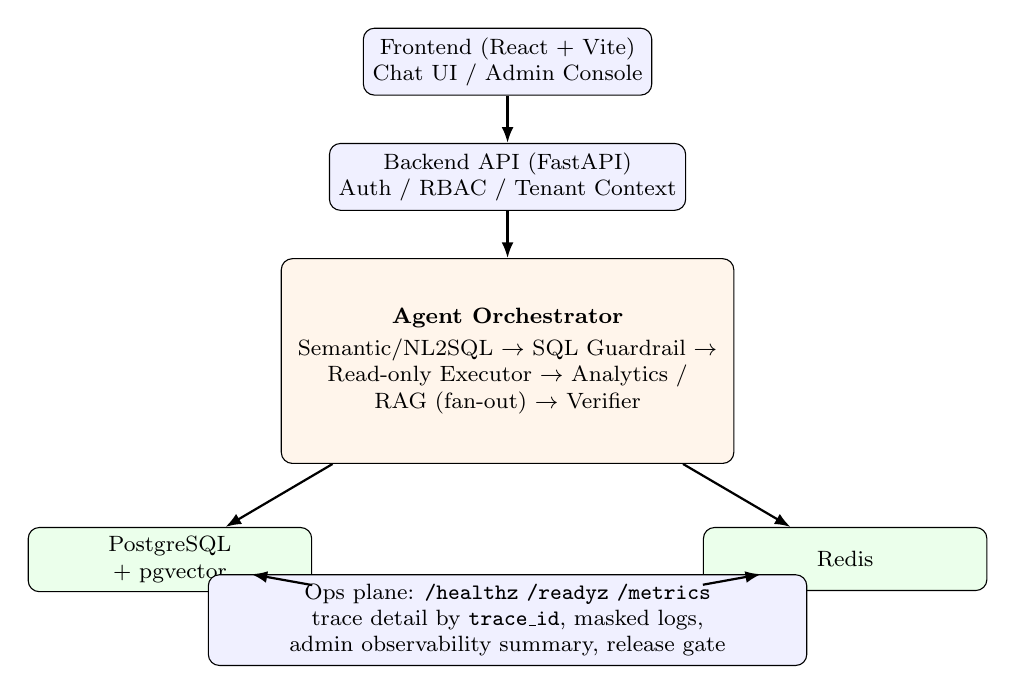
\begin{tikzpicture}[
  node distance=6mm and 8mm,
  box/.style={draw, rounded corners, minimum width=3.6cm, minimum height=0.8cm,
              align=center, font=\footnotesize, fill=blue!6},
  bigbox/.style={draw, rounded corners, minimum width=3.9cm, align=center,
                 font=\footnotesize, fill=orange!8, inner sep=6pt},
  data/.style={draw, rounded corners, minimum width=3.6cm, minimum height=0.8cm,
               align=center, font=\footnotesize, fill=green!8},
  arr/.style={-{Latex[length=2mm]}, thick}
]
\node[box] (fe) {Frontend (React + Vite)\\Chat UI / Admin Console};
\node[box, below=of fe] (api) {Backend API (FastAPI)\\Auth / RBAC / Tenant Context};
\node[bigbox, below=of api, minimum height=2.6cm] (orch) {
  \textbf{Agent Orchestrator}\\[2pt]
  \footnotesize Semantic/NL2SQL $\rightarrow$ SQL Guardrail $\rightarrow$\\
  Read-only Executor $\rightarrow$ Analytics /\\
  RAG (fan-out) $\rightarrow$ Verifier
};
\node[data, below left=8mm and -4mm of orch] (pg) {PostgreSQL\\+ pgvector};
\node[data, below right=8mm and -4mm of orch] (redis) {Redis};
\node[box, below=1.4cm of orch, minimum width=7.6cm] (ops) {
  Ops plane: \texttt{/healthz} \texttt{/readyz} \texttt{/metrics}\\
  trace detail by \texttt{trace\_id}, masked logs,\\
  admin observability summary, release gate
};

\draw[arr] (fe) -- (api);
\draw[arr] (api) -- (orch);
\draw[arr] (orch) -- (pg);
\draw[arr] (orch) -- (redis);
\draw[arr] (pg) -- (ops);
\draw[arr] (redis) -- (ops);
\end{tikzpicture}%
}
\caption{InsightOps AI high-level architecture: request path from the
frontend through auth, orchestration, and the data/operations plane.}
\label{fig:architecture}
\end{figure}

\subsection{Task Classification and Execution Planning}

A \texttt{QuestionClassifier} assigns each question a task type
(\texttt{sql\_query}, \texttt{chart}, \texttt{analytics},
\texttt{rag\_explanation}, \texttt{verification}, or \texttt{file\_data}).
An \texttt{ExecutionPlanBuilder} turns that into an ordered
\texttt{ExecutionPlan} of agent steps grouped into three stages --
\texttt{sql}, \texttt{fanout}, and \texttt{verify} -- each step declaring
its dependencies explicitly. A \texttt{PlanExecutor} runs the plan and
records per-step timing, status, and errors independently of the final
response, so a single agent's failure does not erase visibility into the
steps that succeeded.

\subsection{Governed SQL Model}

SQL generation and SQL execution are deliberately separated by a
non-negotiable guardrail step (Figure~\ref{fig:guardrail}). A candidate SQL
statement produced by the semantic layer is (1) parsed and restricted to a
simple, single-statement \texttt{SELECT} with no DDL/DML; (2) checked
against a table/column allow-list; (3) rewritten to inject a row-count
cap; (4) bounded by a query timeout policy; and only then (5) executed --
and only against a separate, database-level read-only role, not the role
the rest of the application uses. Every decision, allowed or denied, is
written to an audit log keyed by the request's \texttt{trace\_id}, and the
result is masked for personally identifiable fields based on the caller's
permissions before it is returned.

\begin{figure}[t]
\centering
\resizebox{\columnwidth}{!}{%
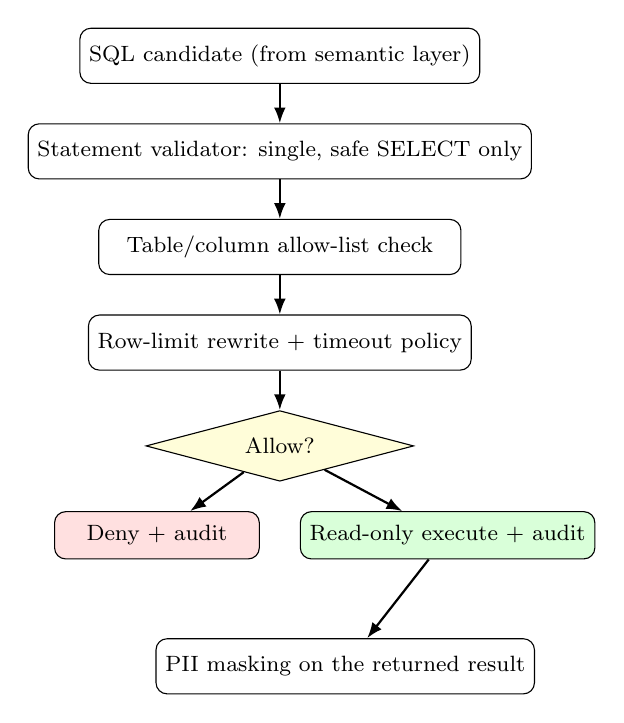
\begin{tikzpicture}[
  node distance=5mm,
  stepbox/.style={draw, rounded corners, minimum width=4.6cm, minimum height=0.7cm,
               align=center, font=\footnotesize},
  decision/.style={draw, diamond, aspect=2.4, minimum width=3.4cm,
                    align=center, font=\footnotesize, fill=yellow!15},
  deny/.style={draw, rounded corners, minimum width=2.6cm, minimum height=0.6cm,
               align=center, font=\footnotesize, fill=red!12},
  allow/.style={draw, rounded corners, minimum width=2.6cm, minimum height=0.6cm,
                align=center, font=\footnotesize, fill=green!15},
  arr/.style={-{Latex[length=2mm]}, thick}
]
\node[stepbox] (cand) {SQL candidate (from semantic layer)};
\node[stepbox, below=of cand] (parse) {Statement validator: single, safe SELECT only};
\node[stepbox, below=of parse] (policy) {Table/column allow-list check};
\node[stepbox, below=of policy] (rewrite) {Row-limit rewrite + timeout policy};
\node[decision, below=of rewrite] (dec) {Allow?};
\node[deny, below left=6mm and -6mm of dec] (deny) {Deny + audit};
\node[allow, below right=6mm and -6mm of dec] (allow) {Read-only execute + audit};
\node[stepbox, below=10mm of allow, minimum width=3.6cm, xshift=-1.3cm] (mask) {PII masking on the returned result};

\draw[arr] (cand) -- (parse);
\draw[arr] (parse) -- (policy);
\draw[arr] (policy) -- (rewrite);
\draw[arr] (rewrite) -- (dec);
\draw[arr] (dec) -- (deny);
\draw[arr] (dec) -- (allow);
\draw[arr] (allow) -- (mask);
\end{tikzpicture}%
}
\caption{SQL guardrail decision pipeline: nothing reaches the database
without clearing every stage, and both outcomes are audited.}
\label{fig:guardrail}
\end{figure}

\subsection{RAG Retrieval Model}

Explanatory questions are answered from real business documents rather
than from the model's own inference. Figure~\ref{fig:rag} shows the
hybrid pipeline: documents are parsed, chunked, embedded, and stored in
pgvector with owner/role metadata; a question is embedded and also scored
lexically with BM25 over the already permission-filtered candidate set;
the two scores are fused, narrowed to a top-$2K$ candidate set, optionally
re-scored by a cross-encoder reranker, and assembled into a
citation-grounded context that the LLM is restricted to answering from.

\begin{figure}[t]
\centering
\resizebox{\columnwidth}{!}{%
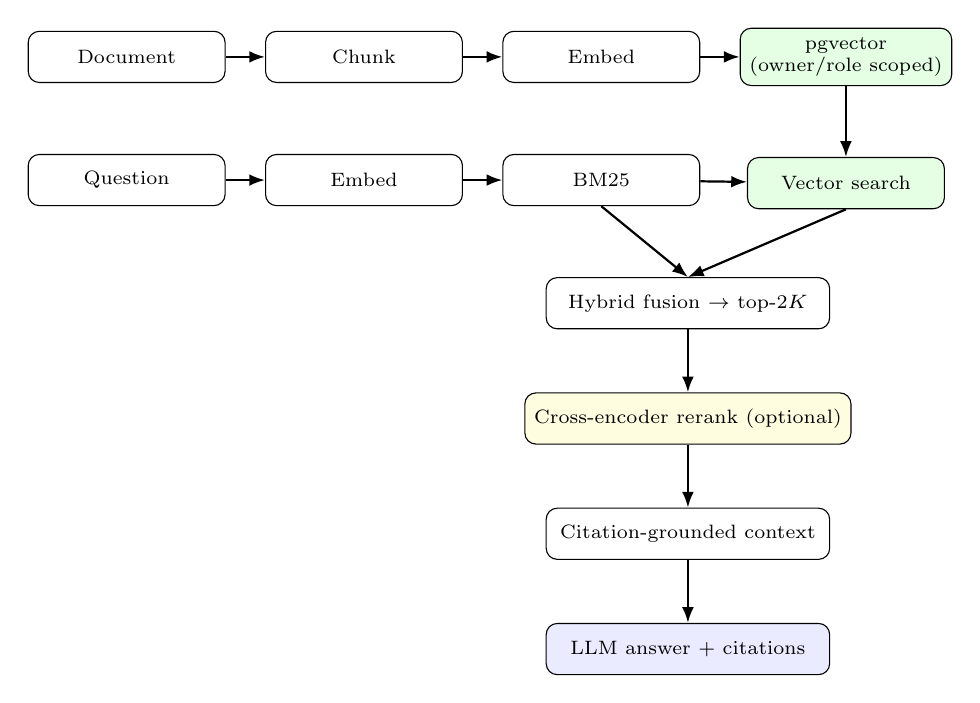
\begin{tikzpicture}[
  node distance=5mm and 5mm,
  stepbox/.style={draw, rounded corners, minimum width=2.5cm, minimum height=0.65cm,
               align=center, font=\scriptsize},
  arr/.style={-{Latex[length=2mm]}, thick}
]
\node[stepbox] (doc) {Document};
\node[stepbox, right=of doc] (chunk) {Chunk};
\node[stepbox, right=of chunk] (embed) {Embed};
\node[stepbox, right=of embed, fill=green!10] (vdb) {pgvector\\(owner/role scoped)};

\node[stepbox, below=9mm of doc] (q) {Question};
\node[stepbox, below=9mm of chunk] (qembed) {Embed};
\node[stepbox, below=9mm of embed] (bm25) {BM25};
\node[stepbox, below=9mm of vdb, fill=green!10] (vsearch) {Vector search};

\node[stepbox, below=9mm of bm25, xshift=1.1cm, minimum width=3.6cm] (fuse) {Hybrid fusion $\rightarrow$ top-$2K$};
\node[stepbox, below=8mm of fuse, minimum width=3.6cm, fill=yellow!12] (rerank) {Cross-encoder rerank (optional)};
\node[stepbox, below=8mm of rerank, minimum width=3.6cm] (ctx) {Citation-grounded context};
\node[stepbox, below=8mm of ctx, minimum width=3.6cm, fill=blue!8] (ans) {LLM answer + citations};

\draw[arr] (doc) -- (chunk);
\draw[arr] (chunk) -- (embed);
\draw[arr] (embed) -- (vdb);
\draw[arr] (q) -- (qembed);
\draw[arr] (qembed) -- (bm25);
\draw[arr] (bm25) -- (vsearch);
\draw[arr] (vdb.south) -- (vsearch.north);
\draw[arr] (bm25.south) -- (fuse.north);
\draw[arr] (vsearch.south) -- (fuse.north);
\draw[arr] (fuse) -- (rerank);
\draw[arr] (rerank) -- (ctx);
\draw[arr] (ctx) -- (ans);
\end{tikzpicture}%
}
\caption{Hybrid RAG pipeline: BM25 keyword scoring and real vector search
are fused, permission-filtered, optionally reranked, and only then handed
to the LLM as a bounded, citable context.}
\label{fig:rag}
\end{figure}

A golden dataset of real, schema-grounded questions with expected chunk
IDs is scored separately with Hit Rate@K and Mean Reciprocal Rank (MRR),
tracked as observability-only metrics until a production baseline exists
to justify a release-gate threshold. This design was itself revised after
a code-level audit found that three of its four documented stages were
placeholders -- a hash-bucket pseudo-embedding standing in for real
vectors on one code path, token-overlap standing in for BM25, and a
``rerank'' step that resorted an already-computed score rather than
running a second model pass. Each gap was written up and closed as a
separate, numbered follow-up design before being implemented, and a
subsequent review pass caught that the reload path was not actually
consuming the backfilled pgvector vectors. That audit trail is kept in the
repository rather than summarized away, because it is stronger evidence of
engineering rigor than a document that only states intentions.

% =============================================================
\section{Detailed Implementation}
\label{sec:implementation}

\subsection{Backend Orchestration}

The backend is a FastAPI application. An application facade coordinates
domain workflows for the orchestrator, and the orchestrator wires together
history, the SQL guardrail, and trace recording. Table~\ref{tab:agents}
lists the agents involved and their single responsibility; each is
independently unit-tested against its own contract rather than only
end-to-end.

\begin{table}[t]
\centering
\caption{Agents and their responsibilities}
\label{tab:agents}
\footnotesize
\begin{tabular}{@{}p{2.1cm}p{5.5cm}@{}}
\toprule
\textbf{Agent} & \textbf{Responsibility} \\
\midrule
SQL Agent & Turns a parsed question into a SQL candidate via the semantic layer and the \texttt{sql\_generation} LLM route \\
SQL Guardrail & Validates, rewrites, and allow/deny-gates every SQL candidate before database access (Fig.~\ref{fig:guardrail}) \\
Read-only Executor & Runs guardrail-approved SQL against the read-only Postgres role \\
Analytics Agent & Forecasting and anomaly detection over the query result \\
Visualization Agent & Produces a chart specification for chart-shaped questions \\
RAG Agent & Runs hybrid retrieval (Fig.~\ref{fig:rag}) for explanatory questions \\
Federated Query Agent & Extends read-only querying to admin-approved business data sources \\
File Data Agent & Answers questions scoped to a user's uploaded file, respecting ownership/sharing \\
Verifier Agent & Checks the assembled answer against its sources before it is returned \\
\bottomrule
\end{tabular}
\end{table}

Confidence is aggregated rather than self-reported: a \texttt{ConfidenceAggregator}
combines signals from the agents that actually ran (SQL success, RAG hit
quality, verifier outcome), weighted per source, instead of trusting a
single model's stated confidence. Long-running analytics/RAG jobs are
handed off through a worker queue to a separate worker process rather than
blocking the chat request.

\subsection{Semantic Layer and NL2SQL}

A semantic catalog constrains what the model is allowed to reference, so
that a term such as ``revenue'' resolves to one agreed metric definition
rather than whatever the model infers from a column name. A question
parser extracts structural intent (metric, dimension, time window,
filters) before generation, and a schema-drift detector flags when the
live database schema has moved away from what the catalog describes. The
NL2SQL step never talks to the database directly; its only output is the
SQL candidate that must clear the guardrail in Figure~\ref{fig:guardrail}.

\subsection{LLM Provider Gateway}

Every model call goes through a single gateway that implements one
provider-agnostic protocol (\texttt{complete(request, route) $\rightarrow$
response}), so timeouts, retries with backoff, and token/cost tracking are
enforced in one place, and providers can be swapped without touching agent
code. Table~\ref{tab:routing} shows the task-based routing model: the
system deliberately makes several smaller model calls per question rather
than one large one, so cheaper/faster models can be routed to
classification while a stronger instruction-following model handles SQL
generation.

\begin{table}[t]
\centering
\caption{Task-based LLM routing}
\label{tab:routing}
\footnotesize
\begin{tabular}{@{}p{2.6cm}p{5cm}@{}}
\toprule
\textbf{Task type} & \textbf{Purpose} \\
\midrule
\texttt{intent\_classification} & Cheap/fast routing of the question to a task type \\
\texttt{sql\_generation} & Strong instruction-following model, grounded in the semantic catalog \\
\texttt{answer\_synthesis} & Grounded only in bounded SQL rows and evidence snippets actually returned upstream \\
\texttt{evidence\_reasoning} & Explanation answers, must cite evidence anchors when available \\
\bottomrule
\end{tabular}
\end{table}

The default provider is a deterministic, network-free mock -- a
deliberate choice, not a placeholder left in by accident, since it is what
allows the automated test and evaluation suite described in
Section~\ref{sec:testing} to run without API cost or dependency on a live
model's uptime. \texttt{OpenAIChatProvider} is the first real adapter,
implemented with the standard library's HTTP client rather than a heavy
SDK dependency, defaulting to \texttt{gpt-4o-mini} as a cost/latency
balance for a workload that issues several model calls per question. The
same reasoning drives the default embedding model,
\texttt{text-embedding-3-small}: 1536 dimensions at low per-token cost,
adequate for chunk-level semantic search where recall matters more than
maximum embedding fidelity. Because both the LLM and embedding clients are
defined as protocols, adding another provider (e.g., Anthropic or Gemini)
is an adapter, not a rewrite of the orchestrator.

\subsection{Frontend}

The frontend is built with React, Vite, and TypeScript, and is compiled to
static assets served by nginx in the Docker Compose deployment. It
includes a chat interface for the primary ChatBI flow and an admin console,
reachable only with the appropriate \texttt{admin:*} permissions, that
surfaces system health, LLM call/token/cost signals, SQL guardrail block
counts, RAG hit rate, evaluation results, and release-gate status.

\subsection{Authentication, RBAC, and Tenant Isolation}

Authentication is implemented, not stubbed: organizations, users with
hashed passwords and a \texttt{token\_version} used for revocation,
short-lived access tokens paired with longer-lived refresh sessions, and a
role-audit-events table recording every permission change with its
before/after state and actor. Admin-only endpoints check specific
permission strings (e.g., \texttt{admin:eval:read}, \texttt{admin:trace:read},
\texttt{admin:audit:read}, \texttt{admin:user:write}) rather than a single
coarse ``is\_admin'' flag, so an organization can, for example, grant
read access to observability data without granting write access to user
roles. Tenant isolation scopes query history, RAG documents/embeddings,
evaluation results, audit logs, and traces by organization; RAG's
owner/role filtering is enforced in the SQL query itself, not applied
after retrieval, which is what closes the class of cross-tenant leak that
application-layer-only filtering would still be vulnerable to.

% =============================================================
\section{Reliability, Governance, and Security}

\subsection{Defense in Depth for SQL Safety}
The guardrail described in Figure~\ref{fig:guardrail} is deliberately not
the only safety layer. Even if the guardrail's own logic had a bug, the
database connection it executes against carries a separate, database-level
read-only role that has no write privileges at all; even if a write
statement somehow slipped past both layers, the object-access allow-list
still bounds which tables and columns are reachable. Every decision --
allowed or denied -- is written to an audit log keyed by the request's
\texttt{trace\_id} and queryable later by an admin.

\subsection{Tenant Isolation as a Query-Level Guarantee}
Rather than trusting an application-layer filter applied after retrieval,
owner/role scoping for RAG documents is pushed into the SQL query against
pgvector itself. This distinction matters: a bug in application-layer
filtering can silently leak a result before the filter runs, while a
query-level constraint cannot return a row that violates it in the first
place. A dedicated test asserts that one tenant cannot retrieve another
tenant's chunks.

\subsection{PII Masking and Audit Trail}
Query results are masked for sensitive fields based on the caller's
permissions after execution, and structured logs mask sensitive content
before it is written. Every guardrail decision, role change, and admin
access to trace/eval/audit data is recorded as an auditable event.

\subsection{Provider Failure Handling}
The LLM gateway enforces a timeout per model call, and retries transient
failures with backoff; a failed SQL-generation call never falls through
to execution, and answer-synthesis failures degrade to returning
structured data rather than an invented summary. Every provider failure
emits an observability event.

\subsection{Evaluation Gates and Human Acceptance}
An evaluation runner scores a suite of cases and produces run/score/failure
records and a report; a release-gate decision combines automated tests,
strict static type checks, and evaluation-quality thresholds into a single
pass/fail signal. A human-acceptance step is required, but deliberately
only \emph{after} the machine gates already pass -- business review can
add judgment on top of a passing state, but it cannot override a failed
one. We consider this an honest constraint on the release process, not an
inconvenience: a system that lets a human override a failing test suite is
not actually gated by that test suite.

% =============================================================
\section{Deployment and DevOps}

\subsection{Local Deployment}
Docker Compose brings up the React frontend, the FastAPI backend, an async
worker, PostgreSQL~16, and Redis~7 with one command. In the default local
mapping, the frontend is reachable at \texttt{http://localhost:8080}, the
backend API at \texttt{http://localhost:8000}, PostgreSQL at
\texttt{localhost:5433}, and Redis at \texttt{localhost:6379}.

\subsection{Cloud Deployment}
A Kubernetes manifest defines the same service topology as a runtime
scaffold, validated by an architecture test that asserts the manifest's
shape rather than deploying it live. This is deliberately presented as a
scaffold rather than a hardened production profile: managed PostgreSQL and
Redis, a real container registry, TLS ingress, a secrets manager, and
horizontal pod autoscaling are documented as the remaining steps rather
than claimed as complete, in the same spirit as being explicit about a
deployment's actual limitations rather than glossing over them.

\subsection{Continuous Integration}
A GitHub Actions workflow runs the release-gate test and type-check bundle
on every push, so the pass/fail signal described in
Section~\ref{sec:testing} is enforced continuously rather than only
checked manually before a demo.

% =============================================================
\section{Testing and Evaluation}
\label{sec:testing}

\subsection{Unit and Integration Tests}
The test suite spans 195 files covering agent contracts, orchestration
routing, guardrail rules, authentication/RBAC/tenant isolation, hybrid RAG
retrieval and scoring, file upload and sharing, frontend state/props
contracts, and Docker/Kubernetes architecture assertions.

\subsection{Static Typing and Architecture Boundaries}
The codebase is checked with \texttt{pyright} in strict mode across both
source and test code, and dedicated architecture-boundary tests assert
that each layer (API, application facade, orchestration, governance,
agents) does not reach past its intended dependencies.

\subsection{Baseline Benchmark Results}
Table~\ref{tab:benchmark} reports the platform's own local,
mock-provider benchmark suite, generated by a reproducible benchmark
script against a fixed commit. These numbers should be read as
reproducible engineering evidence from a deterministic local environment
-- not as production load-test measurements, since they do not exercise a
live LLM provider or a production-scale cluster.

\begin{table}[t]
\centering
\caption{Local baseline benchmark (mock-provider, deterministic)}
\label{tab:benchmark}
\scriptsize
\begin{tabular}{@{}p{1.7cm}p{3.1cm}r@{}}
\toprule
\textbf{Category} & \textbf{Metric} & \textbf{Result} \\
\midrule
Accuracy & Overall evaluation score & 1.0 \\
Accuracy & SQL safety & 1.0 \\
Accuracy & Agent routing & 1.0 \\
Accuracy & RAG faithfulness & 1.0 \\
Detection & Dangerous SQL detection rate (1000 checks) & 1.0 \\
Detection & Benign SQL allow rate (1000 checks) & 1.0 \\
Performance & Guardrail P95 latency (ms) & 0.0546 \\
Concurrency & Chat API success rate (100 req, c=10) & 1.0 \\
Concurrency & Chat API P95 latency (ms) & 70.03 \\
Evaluation & 50-case eval elapsed (ms) & 0.39 \\
Recovery & Retry recovered transient failure & True \\
Recovery & Circuit breaker half-open after cooldown & True \\
Timeout & Slow query denied by timeout policy & True \\
Hallucination & Unsupported-claim rate & 0.1 \\
Hallucination & Ungrounded-answer confidence & 0.5 \\
Observability & Trace lookup P95 (10{,}000 events, ms) & 0.0011 \\
\bottomrule
\end{tabular}
\end{table}

\subsection{Retrieval-Specific Evaluation}
Beyond answer-level scoring, a golden dataset of real, schema-grounded
questions with expected chunk IDs is used to compute Hit Rate@K and MRR
for the retrieval stage specifically -- distinguishing ``did retrieval find
the right evidence'' from ``did the final answer look plausible.'' This is
tracked as an observability-only metric today, pending a production
baseline before a release-gate threshold is set.

% =============================================================
\section{Results and Discussion}

The final version of InsightOps AI achieves the goals set at the start of
the project. First, it supports governed natural-language querying, where
SQL generation and SQL execution are separated by an auditable guardrail
rather than trusted to a single model call. Second, it supports evidence-
grounded explanation through a genuinely hybrid retrieval pipeline, not a
vector-search-only shortcut, with citations and an explicit
missing-evidence signal instead of invented answers. Third, it supports
real security boundaries: authentication, permission-scoped RBAC, and
query-level tenant isolation, rather than a single shared demo login.
Fourth, it supports quality control through an evaluation runner and a
release gate that a human can only accept after, never instead of, the
machine gates passing. Fifth, it is deployable today through Docker
Compose, with a Kubernetes scaffold validated as an architectural shape.

At the same time, several limitations remain. Cloud deployment is a
scaffold, not a hardened managed-cloud production profile; distributed
resilience patterns such as circuit breakers, dead-letter queues, and
load shedding are only partially present; OpenAI is currently the only
real LLM/embedding provider implemented, though the provider protocols
were designed to make adding another one an adapter rather than a
rewrite; the demo/seed data is not yet large enough for realistic
load testing; and the internal trace/log/metric stack has no external
APM exporter yet. We view these as an honest list of remaining
production-hardening work rather than gaps to be minimized in the
description of the system.

Even with these limitations, we believe the project is a meaningful
demonstration of what it takes to make an LLM-backed system trustworthy
for enterprise use: the model's fluency is only half the problem, and the
harder half -- guardrails, auditability, tenant isolation, evaluation
gates, and an honest record of gaps found and closed -- is what this
project spent most of its engineering effort on.

% =============================================================
\section{Individual Contribution}

This was an individually completed project. The author was responsible
for the full scope described in this report: the semantic layer and
governed NL2SQL design, the SQL guardrail and its defense-in-depth model,
multi-agent orchestration and execution planning, the hybrid RAG
retrieval pipeline (including the audit that found and closed its
placeholder stages), the LLM provider gateway and model-selection
rationale, authentication/RBAC/tenant isolation, the evaluation runner and
release gate, the observability stack and its durable-storage/mining
loop, the frontend chat and admin console, the local and Kubernetes
deployment scaffolding, and the accompanying test suite and documentation.

% =============================================================
\section{Conclusion and Future Work}

InsightOps AI treats a natural-language business question as a governed,
multi-agent workflow rather than a single trust-everything model call. The
main lesson of this project is that making an LLM-backed system usable in
an enterprise setting is primarily a governance and systems-engineering
problem, not a prompting problem: the platform is only as trustworthy as
the guardrail standing between the model and the database, the retrieval
pipeline's honesty about what it actually found, and the audit trail that
lets someone explain, after the fact, why an answer was produced.

Future work includes: (1) adding distributed resilience patterns --
circuit breakers, retry queues with dead-letter handling, bulkheads, and
load shedding -- around the LLM gateway and async workers; (2) adding a
second real LLM/embedding provider behind the existing protocol
abstraction to validate that the abstraction holds under a real second
implementation, not just in design; (3) hardening the Kubernetes scaffold
into a managed-cloud production profile with TLS ingress, a secrets
manager, and autoscaling; (4) building a synthetic enterprise-scale
dataset generator to validate the platform under realistic load; and
(5) connecting the existing internal observability stack to an external
APM/metrics backend for production-grade monitoring.

% =============================================================
\begin{thebibliography}{9}
\bibitem{fastapi} FastAPI, ``FastAPI Documentation.'' [Online]. Available: \url{https://fastapi.tiangolo.com/}
\bibitem{pgvector} pgvector, ``pgvector: Open-source vector similarity search for Postgres.'' [Online]. Available: \url{https://github.com/pgvector/pgvector}
\bibitem{redis} Redis, ``Redis Documentation.'' [Online]. Available: \url{https://redis.io/docs/}
\bibitem{openai} OpenAI, ``OpenAI API Reference.'' [Online]. Available: \url{https://platform.openai.com/docs/}
\bibitem{bm25} S. Robertson and H. Zaragoza, ``The Probabilistic Relevance Framework: BM25 and Beyond,'' \emph{Foundations and Trends in Information Retrieval}, vol. 3, no. 4, pp. 333--389, 2009.
\bibitem{k8s} Kubernetes, ``Kubernetes Documentation.'' [Online]. Available: \url{https://kubernetes.io/docs/}
\bibitem{react} React, ``React Documentation.'' [Online]. Available: \url{https://react.dev/}
\end{thebibliography}

\end{document}
